\chapter{الهندسة الوراثية والتقانة الحيوية}\label{ch:b3:genetic-engineering}

حتى عام 1982 كان كل مصاب بالسكري في العالم يبقى حيًا بأنسولين
مستخلص من بنكرياس الخنازير والأبقار --- نحو ثمانية آلاف كيلوغرام من
الغدد لكيلوغرام واحد من الهرمون --- وكانت نسبة من المرضى تتحسس من
البروتين الغريب. وفي تلك السنة بلغ السوقَ أول دواء صنعه كائن
مهندَس وراثيًا: أنسولين بشري تركّبه \emph{Escherichia coli} حاملةً
المورّثة البشرية على \omterm{def:b3:genetic-engineering:tools}{بلازميد}. وكانت الأدوات التي أتاحت ذلك قد
جُمعت في العقد السابق --- إنزيمات تقطع DNA عند متتاليات
مختارة، وإنزيمات تصل القطع، وبلازميدات تحملها إلى
خلية وتنسخها فيها --- وانضم إليها في العقود التالية
\omterm{def:b3:genetic-engineering:pcr}{تفاعل البوليميراز المتسلسل}، وحقن المورّثات في الأجنّة،
ومنذ عام 2012 منظومة مناعية بكتيرية حُوّلت إلى مقص
قابل للبرمجة يستطيع إعادة كتابة حرف واحد من جينوم
في خلية حية. وهذا الفصل عن تلك الأدوات، وعن الحساب
الذي يحكم استعمالها، وما بُني بها، من فأر
متوهج إلى شفاء من فقر الدم المنجلي.

\section{قطع DNA ووصله ونسخه}

\begin{definition}[إنزيمات القطع، والليغاز، والنواقل]\label{def:b3:genetic-engineering:tools}
\index{إنزيم قطع}\index{نهاية لزجة}\index{ليغاز DNA}\index{ناقل}\index{بلازميد}\index{واسم انتقائي}
\emph{إنزيم القطع} من النمط~II نوكلياز داخلي بكتيري
يقطع DNA المزدوج الطاق عند متتالية بعينها من \numrange{4}{8}
أزواج قواعد، متناظرة عادةً: فإنزيم EcoRI يقطع G$^{\downarrow}$AATTC،
تاركًا نتوءات مفردة الطاق من أربع قواعد (\emph{نهايات لزجة})
متممة لأي نهاية EcoRI أخرى؛ وإنزيمات أخرى تترك \emph{نهايات
كليلة}. و\emph{ليغاز DNA} يختم قطعتين تتوافق نهاياتهما. و
\emph{الناقل} جزيء DNA يتضاعف في مضيف ويستطيع أن يحمل
قطعة مقحمة: ومنه \emph{البلازميد} ذو بضع كيلوقواعد وفيه
مَنشأ تضاعف، و\emph{واسم انتقائي} (مورّثة مقاومة
لمضاد حيوي، فلا ينمو على المضاد إلا الخلايا التي التقطت
البلازميد) وعنقود من مواقع قطع فريدة
للمقحَمة؛ ومنها أيضًا العاثية $\lambda$، والكوزميدات، والصبغيات
الاصطناعية البكتيرية أو الخميرية لمقحمات من \qtyrange{20}{1000}{kb}. ويدخل DNA
البكتيريا عبر \emph{التحول}، بعد صدمة كيميائية أو
كهربائية تجعل الغشاء نفوذًا عابرًا، بكفاءة
من $10^{6}$ إلى $10^{9}$ متحوّل لكل ميكروغرام من
البلازميد. والجزيء \emph{المؤتلف} هو الذي يصل DNA من
مصدرين.
\end{definition}

\begin{proof}[شواهد]
قطع كوهن وتشانغ وبوير وهيلينغ (1973) \omterm{def:b3:genetic-engineering:tools}{البلازميد} pSC101 وبلازميدًا
ثانيًا يحمل مورّثة مقاومة أخرى بإنزيم EcoRI، ومزجوا
القطع ووصلوها، وحوّلوا \emph{E.~coli}، واستخرجوا
مستعمرات مقاومة للمضادين معًا تحمل بلازميدًا واحدًا مصنوعًا من
كليهما --- وهو أول DNA مؤتلف يتضاعف في خلية. وفي السنة التالية
أقحموا مورّثات RNA الريبوزومي لضفدع في pSC101 وبيّنوا أن
DNA الضفدع تضاعف واستُنسخ في البكتيريا: فالمورّثات
تعبر الحد بين الممالك بلا تغير، والبكتيريا
تنسخ أي DNA يُعطى لها.
\end{proof}

\begin{omfigure}
\begin{tikzpicture}[every node/.style={font=\scriptsize}, >=stealth]
  % plasmid circle
  \draw[very thick, omDef] (0,0) circle (1.8);
  % ori
  \draw[very thick, omMeth!70!black] (0,0) ++(60:1.8) arc[start angle=60, end angle=100, radius=1.8]; \node[above right] at (80:1.95) {منشأ التضاعف};
  % ampR
  \draw[very thick, omProp] (0,0) ++(160:1.8) arc[start angle=160, end angle=250, radius=1.8]; \node[left, align=right] at (205:2.0) {مورّثة المقاومة\\وهي الواسم};
  % MCS with insert
  \draw[very thick, omThm] (0,0) ++(-40:1.8) arc[start angle=-40, end angle=10, radius=1.8]; \node[right, align=left] at (-15:2.0) {المقحَمة، موصولةً في\\موقع القطع};
  \draw[omThm] (-40:1.7) -- (-40:1.95); \draw[omThm] (10:1.7) -- (10:1.95);
  \node at (0,0.25) {بلازميد}; \node at (0,-0.15) {\qtyrange{3}{5}{kb}};
  % sticky ends detail
  \begin{scope}[xshift=5.7cm, yshift=0.8cm]
    \node[left, align=right] at (-0.2,0) {EcoRI};
    \node[font=\ttfamily\scriptsize, anchor=west] at (0,0.25) {5$'$-G\,\textcolor{omThm}{AATT}C-3$'$};
    \node[font=\ttfamily\scriptsize, anchor=west] at (0,-0.25) {3$'$-C\textcolor{omThm}{TTAA}\,G-5$'$};
    \draw[->, omThm, thick] (0.62,0.55) -- (0.62,0.3); \draw[->, omThm, thick] (1.62,-0.55) -- (1.62,-0.3);
    \node[anchor=west, align=left] at (2.9,0) {قطوع متدرجة تترك\\نتوءات متممة من أربع\\قواعد: نهايات لزجة};
  \end{scope}
  \begin{scope}[xshift=5.7cm, yshift=-1.3cm]
    \draw[very thick, omDef] (0,0.15) -- (1.2,0.15); \draw[very thick, omDef] (0,-0.15) -- (0.7,-0.15);
    \draw[very thick, omThm] (1.7,0.15) -- (3.0,0.15); \draw[very thick, omThm] (1.2,-0.15) -- (3.0,-0.15);
    \node[above] at (1.45,0.2) {تلاحم}; \node[below, align=center] at (1.5,-0.25) {أي نهايتي EcoRI تزدوجان؛\\والليغاز يختم الهيكل};
  \end{scope}
\end{tikzpicture}

{\small \omterm{def:b3:genetic-engineering:tools}{ناقل} استنساخ وكيمياؤه. يحمل \omterm{def:b3:genetic-engineering:tools}{البلازميد}
منشأً، وواسمًا انتقائيًا، وموقع قطع فريدًا تُوصل فيه
قطعة قُطعت بالإنزيم نفسه؛ والنهايات اللزجة تجعل أي قطعتين
قطعهما الإنزيم نفسه متوافقتين.}
\end{omfigure}

\begin{method}[استنساخ مورّثة]\label{met:b3:genetic-engineering:cloning}
\index{استنساخ}\index{مكتبة}\index{فرز}
(1) احصل على المقحَمة: اقطع DNA الجينومي \omterm{def:b3:genetic-engineering:tools}{بإنزيم قطع}، أو
انسخ RNA الرسول إلى DNA متمم (cDNA، وهو يخلو من الإنترونات
فيمكن التعبير عنه في البكتيريا)، أو ضخّم المورّثة بتفاعل PCR
ببادئتين تحملان مواقع قطع. (2) اقطع \omterm{def:b3:genetic-engineering:tools}{الناقل} والمقحَمة بالإنزيم
(أو الإنزيمين) نفسه --- وإنزيمان مختلفان يفرضان اتجاه المقحَمة
--- ثم صِلْهما. (3) حوّل البكتيريا وازرعها على المضاد الحيوي:
فلا ينمو إلا ما فيه \omterm{def:b3:genetic-engineering:tools}{بلازميد}. (4) ميّز البلازميدات ذات المقحَمة
من التي انغلقت على نفسها: بمورّثة واسمة يقطعها موقع
الاستنساخ (\emph{lacZ}: فالمستعمرات البيضاء فيها مقحَمة والزرقاء لا).
(5) افرز المستعمرات بحثًا عن المقحَمة المطلوبة: بالتهجين بمسبار
موسوم، أو بتفاعل PCR، أو بالهضم بإنزيمات القطع والترحيل
الكهربائي على هلام. (6) سلسِل المقحَمة. و\emph{المكتبة} هي
مجموعة النسائل من جينوم كامل أو منسوخ كامل، يمكن أن تُصاد منها
أي مورّثة بالفرز نفسه.
\end{method}

\begin{omfigure}
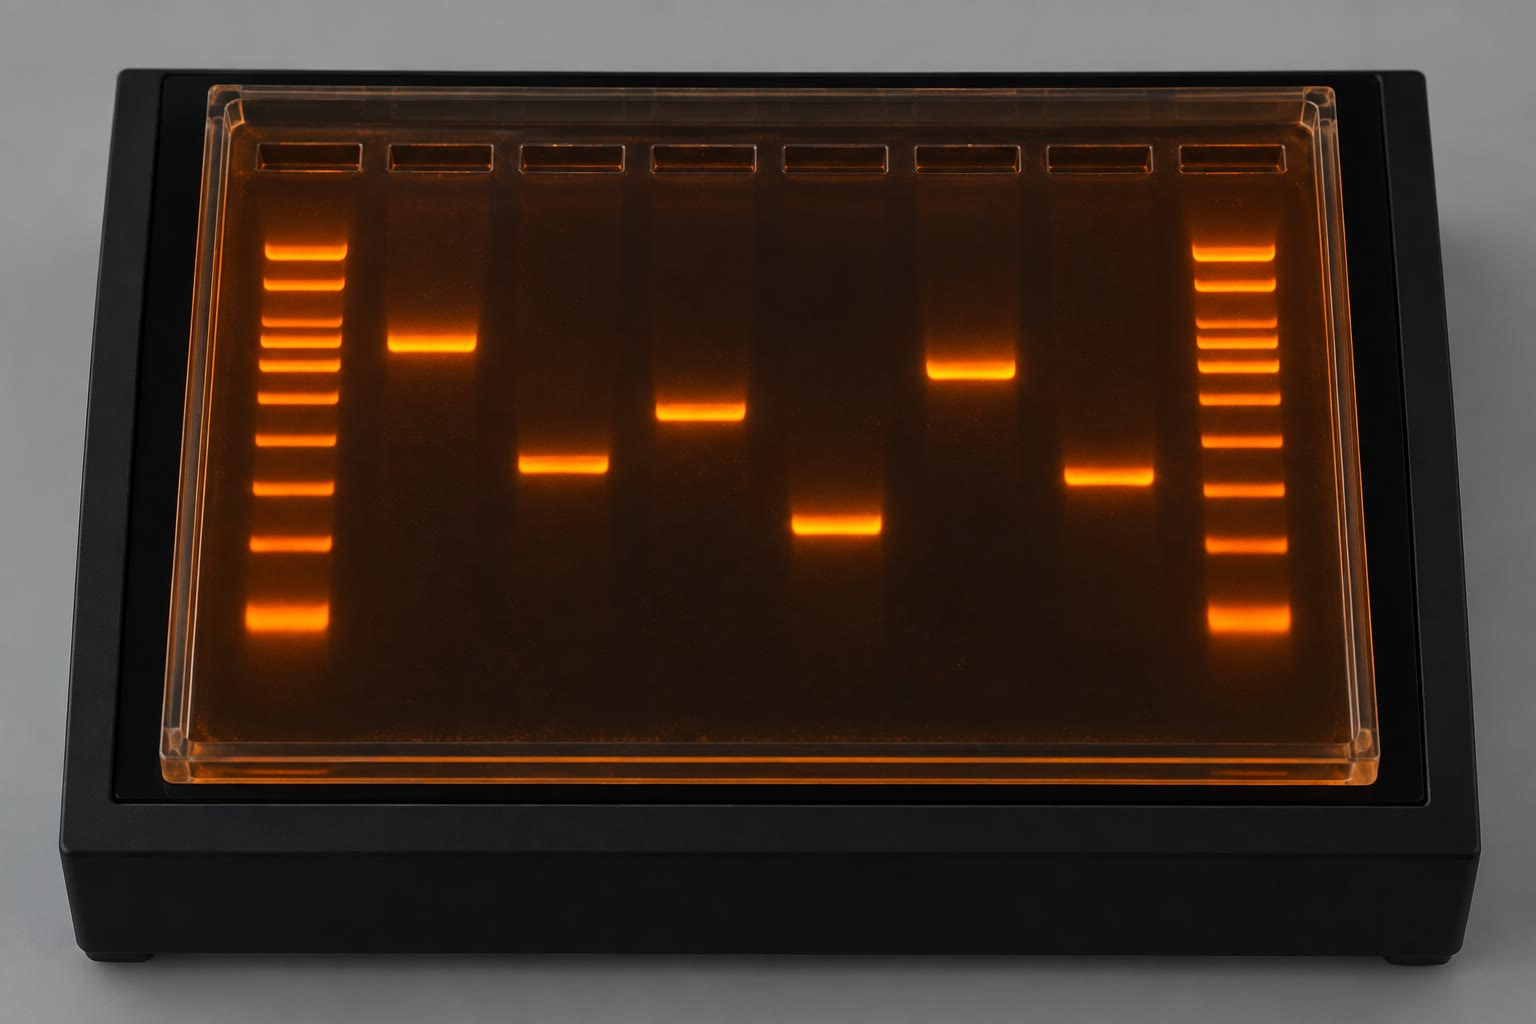
\includegraphics[width=0.56\linewidth]{images/book5/ai/b5-06-agarose-gel.jpg}

{\small هلام أغاروز تحت الضوء فوق البنفسجي: تهاجر قطع DNA
نحو المصعد بسرعة تتناقص مع طولها، فتكون كل حزمة
جمهرةً من جزيئات ذات حجم واحد، تُقارن بسلّم
الأحجام المعلومة في المسربين الخارجيين.}
\end{omfigure}

\begin{definition}[تفاعل البوليميراز المتسلسل]\label{def:b3:genetic-engineering:pcr}
\index{تفاعل البوليميراز المتسلسل}\index{بادئة}\index{PCR كمي}
\emph{تفاعل البوليميراز المتسلسل} (PCR) يضخّم قطعة مختارة
من DNA بين \emph{بادئتين} --- وهما قليلا نوكليوتيد مركّبان من
نحو عشرين قاعدة متممين للطاقين عند طرفي
الهدف --- عبر دورات من ثلاث درجات حرارة: \qty{95}{\celsius}
لفصل الطاقين، و\qtyrange{50}{65}{\celsius} لتلاحم البادئتين،
و\qty{72}{\celsius} ليستطيلهما بوليميراز ثابت حراريًا (Taq، من
بكتيريا الينابيع الحارة \emph{Thermus aquaticus}). وكل
دورة تضاعف عدد نسخ القطعة الواقعة بين البادئتين،
فتحوّل ثلاثون دورة جزيئًا واحدًا إلى مليار. و\emph{تفاعل PCR
مع النسخ العكسي} ينسخ RNA أولًا إلى DNA فيقيس
النسخ أو فيروسات RNA؛ و\emph{تفاعل PCR الكمي} (qPCR) يتابع
التضخيم في الزمن الحقيقي بصبغ متألق ويقرأ
الكمية الابتدائية من الدورة التي تعبر عندها الإشارة
عتبةً.
\end{definition}

\begin{theorem}[حساب التضخيم]\label{thm:b3:genetic-engineering:pcr}
\index{دورة العتبة}
بكفاءة $E$ لكل دورة ($E = 1$ للمضاعفة التامة)، تصير $N_{0}$
نسخة ابتدائية
\[
N_{n} = N_{0}\,(1 + E)^{n}
\]
بعد $n$ دورة. وإذا عبر التألق عتبةً ثابتة حين
يبلغ عدد النسخ $N_{T}$، كانت \emph{\omterm{thm:b3:genetic-engineering:pcr}{دورة العتبة}}
\[
C_{T} = \frac{\log N_{T} - \log N_{0}}{\log(1 + E)},
\]
وهي خط مستقيم في $\log N_{0}$ ميله $-1/\log(1+E)$: فعند $E = 1$
يخفض كل ازدياد عشري في الكمية الابتدائية $C_{T}$ بمقدار
$\log_{2} 10 = 3.32$ دورة، وعينتان تختلف دورتا عتبتهما
بمقدار $\Delta C_{T}$ تختلفان في النسخ الابتدائية بالعامل
$(1 + E)^{\Delta C_{T}}$.
\end{theorem}
\begin{proof}
كل دورة تضرب عدد النسخ في $1 + E$، فتكون $N_{n}$
متتالية هندسية. ووضع $N_{n} = N_{T}$ والحل من أجل $n$ يعطي
$C_{T}$؛ والميل معامل $\log N_{0}$. ولعينتين،
$C_{T,1} - C_{T,2} = (\log N_{0,2} - \log N_{0,1})/\log(1+E)$، ومنه
$N_{0,2}/N_{0,1} = (1+E)^{\Delta C_{T}}$.
\end{proof}

\begin{example}[قراءة لوحة qPCR]\label{ex:b3:genetic-engineering:qpcr}
اختبار لجزيء RNA فيروسي يعبر العتبة عند الدورة $22$ عند مريض
وعند الدورة $32$ عند آخر؛ وعند $E \approx 1$ يحمل الأول $2^{10}
\approx 1000$ ضعف الفيروس. وعينة من عشر نسخ تعبر عند
الدورة $37$ تقريبًا حين تكون العتبة $10^{12}$ نسخة ($\log_{2} 10^{11} =
36.5$)؛ فشوط من $40$ دورة يكشف إذن بضعة جزيئات، ويكشف
كذلك جزيئًا ملوثًا واحدًا من ناتج تضخيم سابق، ولهذا
تفصل المختبرات الغرف التي يُهيَّأ فيها التفاعل عن تلك التي
تُعالَج فيها النواتج.
\end{example}

\begin{omfigure}
\begin{tikzpicture}
\begin{axis}[
  width=0.7\linewidth, height=5.6cm,
  axis x line=bottom, axis y line=left,
  xmin=0, xmax=40, ymin=1, ymax=1e14, ymode=log,
  xlabel={الدورة}, ylabel={النسخ},
  xlabel style={font=\small, at={(axis description cs:0.5,-0.12)}, anchor=north},
  ylabel style={font=\small},
  tick label style={font=\small}, xtick={0,10,20,30,40},
  clip=false,
]
\addplot[very thick, omDef, domain=0:40, samples=41] {1e7*2^x/(1+2^x/1e5)};
\addplot[very thick, omThm, domain=0:40, samples=41] {1e4*2^x/(1+2^x/1e8)};
\addplot[very thick, omMeth!70!black, domain=0:40, samples=41] {10*2^x/(1+2^x/1e11)};
\addplot[dashed, gray, domain=0:40, samples=2] {1e12};
\node[font=\scriptsize, gray, anchor=south west] at (axis cs:0.5,1.3e12) {العتبة $N_{T}$};
\draw[gray] (axis cs:16.6,1) -- (axis cs:16.6,1e12); \draw[gray] (axis cs:26.6,1) -- (axis cs:26.6,1e12); \draw[gray] (axis cs:36.5,1) -- (axis cs:36.5,1e12);
\node[font=\scriptsize, anchor=south] at (axis cs:16.6,3e12) {$C_{T} = 16.6$}; \node[font=\scriptsize, anchor=south] at (axis cs:26.6,3e12) {$26.6$}; \node[font=\scriptsize, anchor=south] at (axis cs:36.5,3e12) {$36.5$};
\end{axis}
\end{tikzpicture}

{\small منحنيات التضخيم عند $N_{0} = 10^{7}$ (بالأزرق) و$10^{4}$ (بالأحمر)
و$10$ نسخ (بالأخضر)، عند $E = 1$، مع الهضبة التي تفرضها الكواشف. ففرق بألف ضعف في
$N_{0}$ يزيح \omterm{thm:b3:genetic-engineering:pcr}{دورة العتبة} بمقدار $10$؛ والهضاب كلها متشابهة،
ولهذا لا يقول الناتج النهائي شيئًا عن البداية.}
\end{omfigure}

\section{صنع البروتينات}

\begin{definition}[منظومات التعبير]\label{def:b3:genetic-engineering:expression}
\index{ناقل تعبير}\index{بروتين مؤتلف}\index{جسم مضاد وحيد النسيلة}
\emph{\omterm{def:b3:genetic-engineering:tools}{ناقل} التعبير} يضع المتتالية المشفِّرة المستنسخة تحت
مروّج قوي قابل للتحكم من المضيف (مروّج \emph{lac} أو T7
في \emph{E.~coli}، يحرّضه نظير سكري)، مع
موقع ربط ريبوزومي، ومنهٍ، وغالبًا \emph{وسم} --- ستة
هستيدينات، أو بروتين صغير --- ملحوم بالناتج لتنقيته
على عمود. والبكتيريا تصنع غرامات في اللتر من بروتين بسيط
(الأنسولين، وهرمون النمو، والإنزيمات) لكنها لا تستطيع غلكزة
بروتينات الثدييات المعقدة ولا طيّها؛ والخميرة تضيف سكريات من نوعها هي؛ وخلايا
الحشرات والثدييات (وخلايا مبيض الهامستر الصيني هي معيار الصناعة)
تصنع الأجسام المضادة وعوامل التخثر مطويةً ومغلكزة
كما في الإنسان. و\emph{الجسم المضاد وحيد النسيلة} يصنعه
\emph{هجين ورمي} --- خلية B منتجة للأجسام المضادة ملحومة بخلية
نقيّية خالدة (كوهلر وميلشتاين، 1975) --- أو، اليوم، باستنساخ
مورّثات الجسم المضاد في خط تعبير ثديي، حيث يمكن استبدال
هيكل الفأر بتسلسل بشري لتجنب الرفض المناعي
(\cref{ch:b3:adaptive-immunity}).
\end{definition}

\begin{example}[الأنسولين]\label{ex:b3:genetic-engineering:insulin}
الأنسولين البشري سلسلتان، A (21 بقية) وB (30)، تصلهما
روابط ثنائية الكبريت، وتُقطعان في الخلية $\beta$ من طليعة
أنسولين واحدة. وقد عبّرت أول عملية عن السلسلتين منفصلتين في
\emph{E.~coli}، كل منهما ملحومة بإنزيم $\beta$-غلاكتوزيداز، ثم شُطرتا
كيميائيًا ووُصلتا خارج الجسم؛ أما العمليات اللاحقة فتعبّر عن طليعة الأنسولين
وتشطرها بالإنزيمات التي يستعملها البنكرياس. ومنذ عام 1996
غُيّر التسلسل نفسه: فإبدال بقية أو اثنتين أو إضافتهما
يعطي نظائر تتفكك أسرع (لوجبة) أو تترسب عند
موضع الحقن وتُطلق على مدى يوم. فالبروتين الذي كان يقتضي ثماني
أطنان من الغدد لكل كيلوغرام يُصنع اليوم في مخمّرة، مطابقًا
للبشري أو أفضل منه.
\end{example}

\section{الكائنات النقيلة}

\begin{definition}[التنقيل والاستهداف المورّثي]\label{def:b3:genetic-engineering:transgenic}
\index{كائن نقيل}\index{حقن مجهري}\index{حذف مورّثي}\index{خلية جذعية جنينية}\index{استهداف مورّثي}
الكائن \emph{النقيل} يحمل مورّثة أُدخلت في سلالته
الجنسية، فتكون في كل خلية وتُورَّث. وفي الفئران
الطريق التقليدي هو \emph{الحقن المجهري} لجزيء DNA في إحدى النواتين الأوليتين
لبيضة ملقحة (غوردون ورادل، 1980)، فيندمج عند
موضع عشوائي في نسبة من الأجنّة؛ وصنع بالميتر وبرينستر (1982)
فئرانًا ضعف الحجم السوي بحقن مورّثة هرمون نمو الجرذ خلف
مروّج ميتالوثيونين. أما \emph{الاستهداف المورّثي} فيستبدل مورّثة
مختارة أو يعطّلها بدل ذلك: إذ تُدخل بنية ذات ذراعين طويلتين متماثلتين مع
الهدف في \emph{خلايا جذعية جنينية}، وتُنتقى الخلايا النادرة
التي وضعتها فيها إعادةُ التركيب المتماثلة في الموضع الصحيح
وتُحقن في كيسة أريمية، فينقل الفأر الخيمري
الناتج المورّثة المبدَّلة (كابيتشي وسميثيز وإيفانز،
في ثمانينيات القرن العشرين). و\emph{الحذف} يفقد المورّثة؛ و\emph{الإدخال} يحمل
نسخة معدَّلة؛ و\emph{الأليل الشرطي}، المحفوف بموقعي loxP،
لا يُحذف إلا حيث ومتى يُعبَّر عن Cre
(\cref{ch:b3:dna-repair}). وقد حُذفت نحو عشرة آلاف مورّثة فأرية،
وكان النمط الظاهري في معظمها أول دليل على
ما تفعله المورّثة.
\end{definition}

\begin{omfigure}
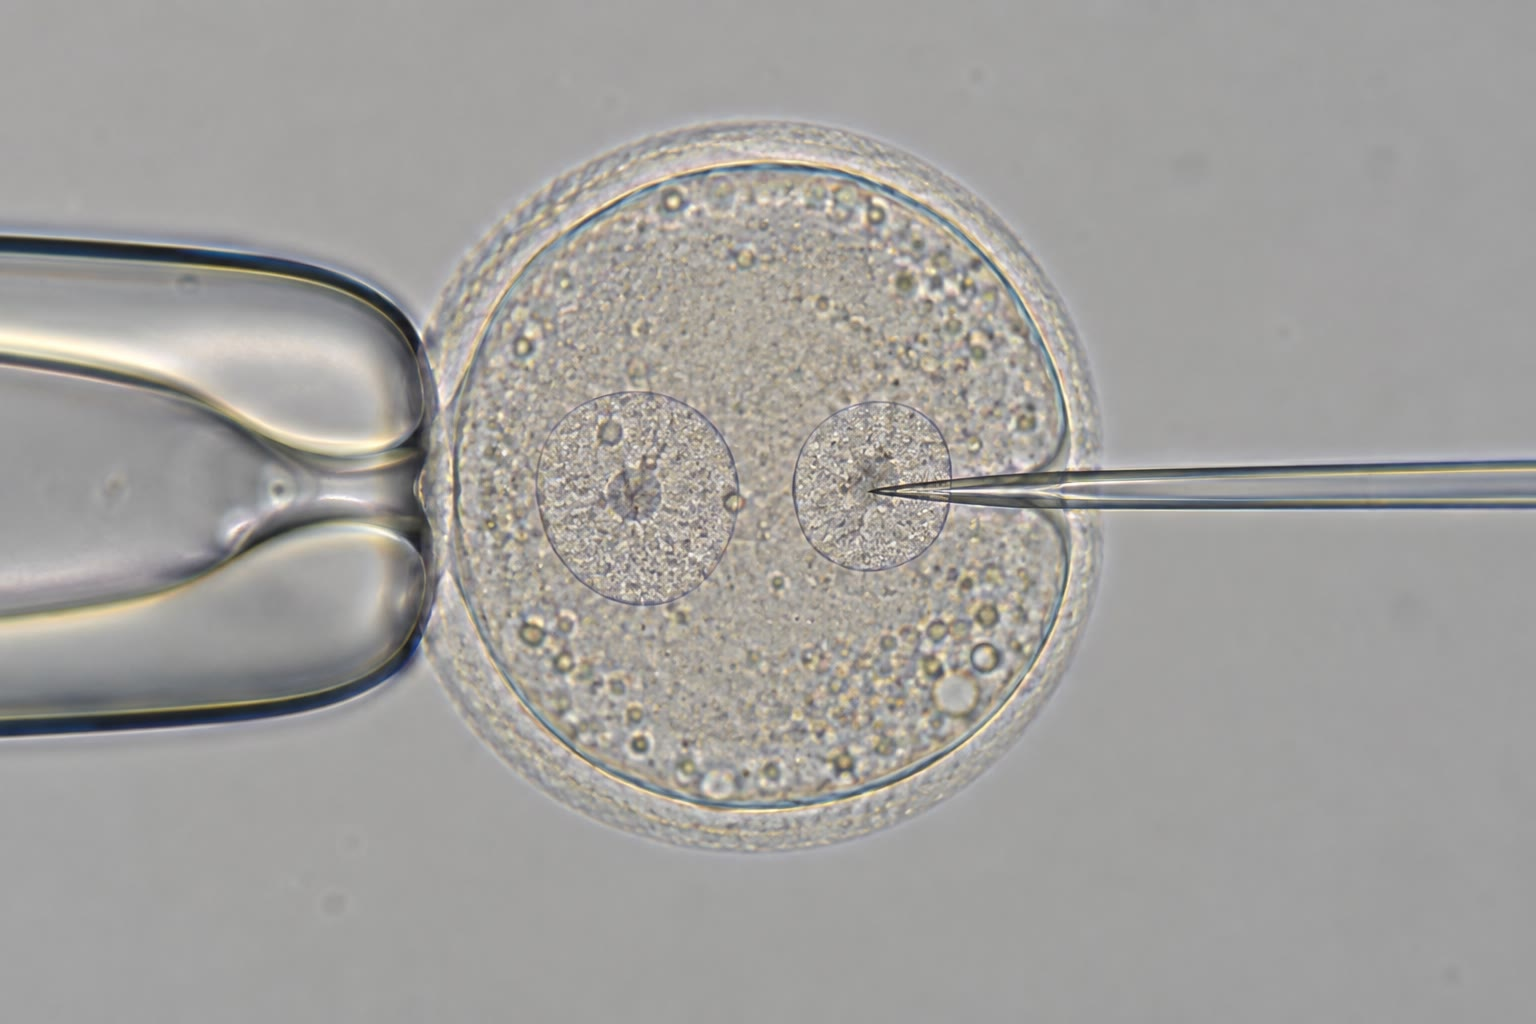
\includegraphics[width=0.46\linewidth]{images/book5/ai/b5-06-microinjection.jpg}\hspace{0.04\linewidth}
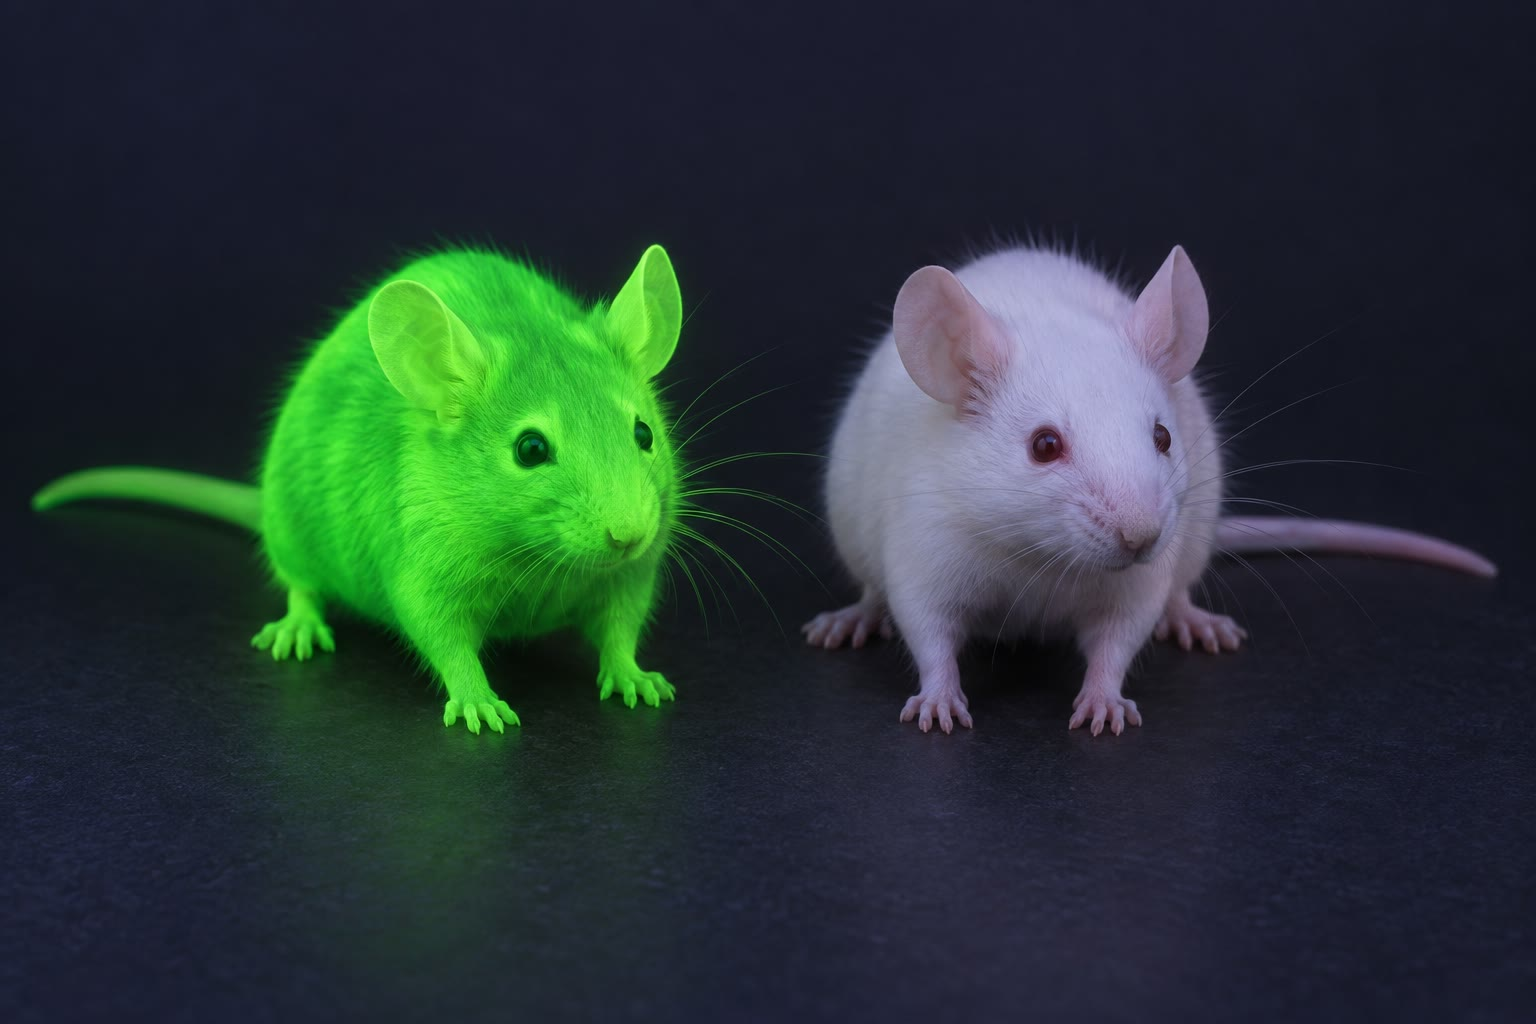
\includegraphics[width=0.46\linewidth]{images/book5/ai/b5-06-gfp-mouse.jpg}

{\small يسارًا: بيضة فأرة ملقحة ممسوكة بالمصّ بينما تحقن
إبرة زجاجية DNA في إحدى نواتيها الأوليتين. يمينًا: فأر نقيل
يعبّر عن البروتين الأخضر المتألق لقنديل بحر في كل خلية،
بجانب أخيه العادي من البطن نفسها، تحت الضوء فوق البنفسجي.}
\end{omfigure}

\begin{definition}[النباتات النقيلة]\label{def:b3:genetic-engineering:plants}
\index{Agrobacterium}\index{T-DNA}\index{محصول معدَّل وراثيًا}
تُحوَّل النباتات ببكتيريا \emph{Agrobacterium tumefaciens}، وهي بكتيريا
تربة تقحم طبيعيًا قطعة من بلازميدها المحدث
للأورام، وهي \emph{T-DNA}، في جينوم نبات مجروح لتجعله
ينمّي دَرَنة ويغذي البكتيريا. واستبدال مورّثات T-DNA نفسها
بأي مورّثة مختارة، بين المتتاليتين الحديّتين اللتين تتعرفهما البكتيريا،
يحوّل الممرض ناقلًا؛ وتُنتقى الخلايا المحوَّلة
وتُجدَّد نباتات كاملة، وكل خلية نباتية تستطيع ذلك. أما
الأنواع التي لا تصيبها البكتيريا (والحبوب زمنًا
طويلًا) فتُحوَّل بقذف جسيمات ذهبية مغلفة بجزيء DNA في
نسيجها. و\emph{المحاصيل المعدَّلة وراثيًا} المزروعة على نطاق واسع تحمل
مورّثة ذيفان بكتيري (\emph{Bt}) ضد يرقات الحشرات، أو إنزيمًا
بكتيريًا يمنح تحملًا لمبيد أعشاب، أو كليهما؛ و\emph{الأرز الذهبي}
يحمل مورّثتين من مسلك الكاروتينويد (سينثاز فيتوئين نباتي
ونازع إشباع بكتيري) حتى تصنع سويداؤه
$\beta$-كاروتين، وهو طليعة الفيتامين~A، الذي يُعمي عوزُه
ويقتل مئات الآلاف من الأطفال كل سنة.
\end{definition}

\begin{omfigure}
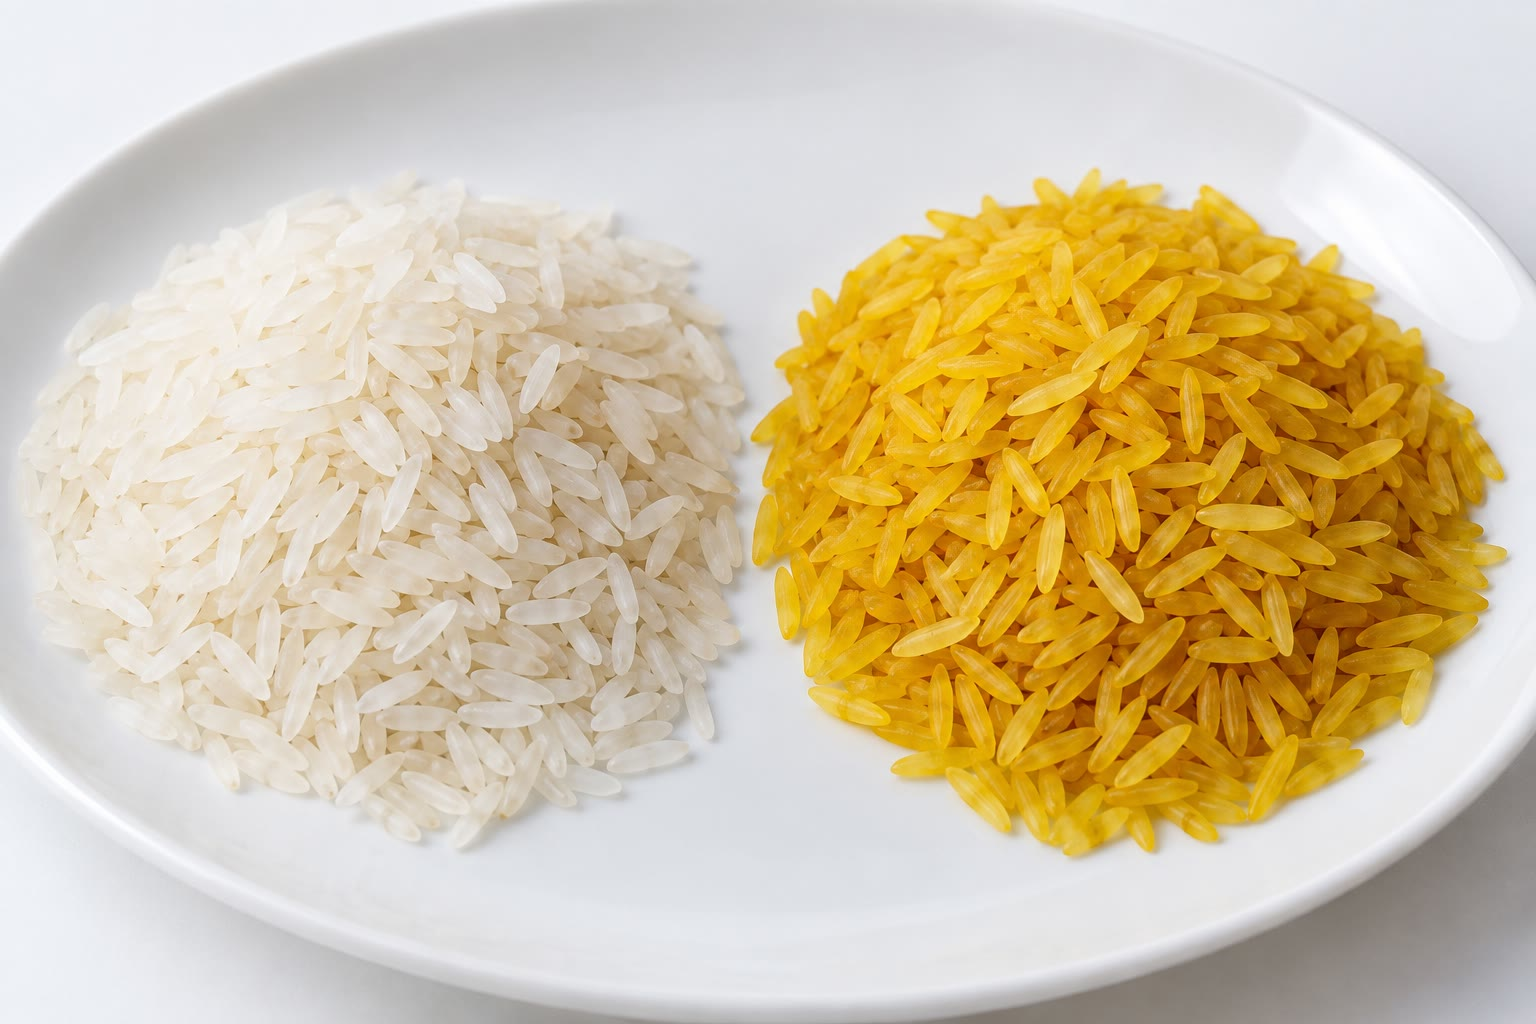
\includegraphics[width=0.46\linewidth]{images/book5/ai/b5-06-golden-rice.jpg}\hspace{0.04\linewidth}
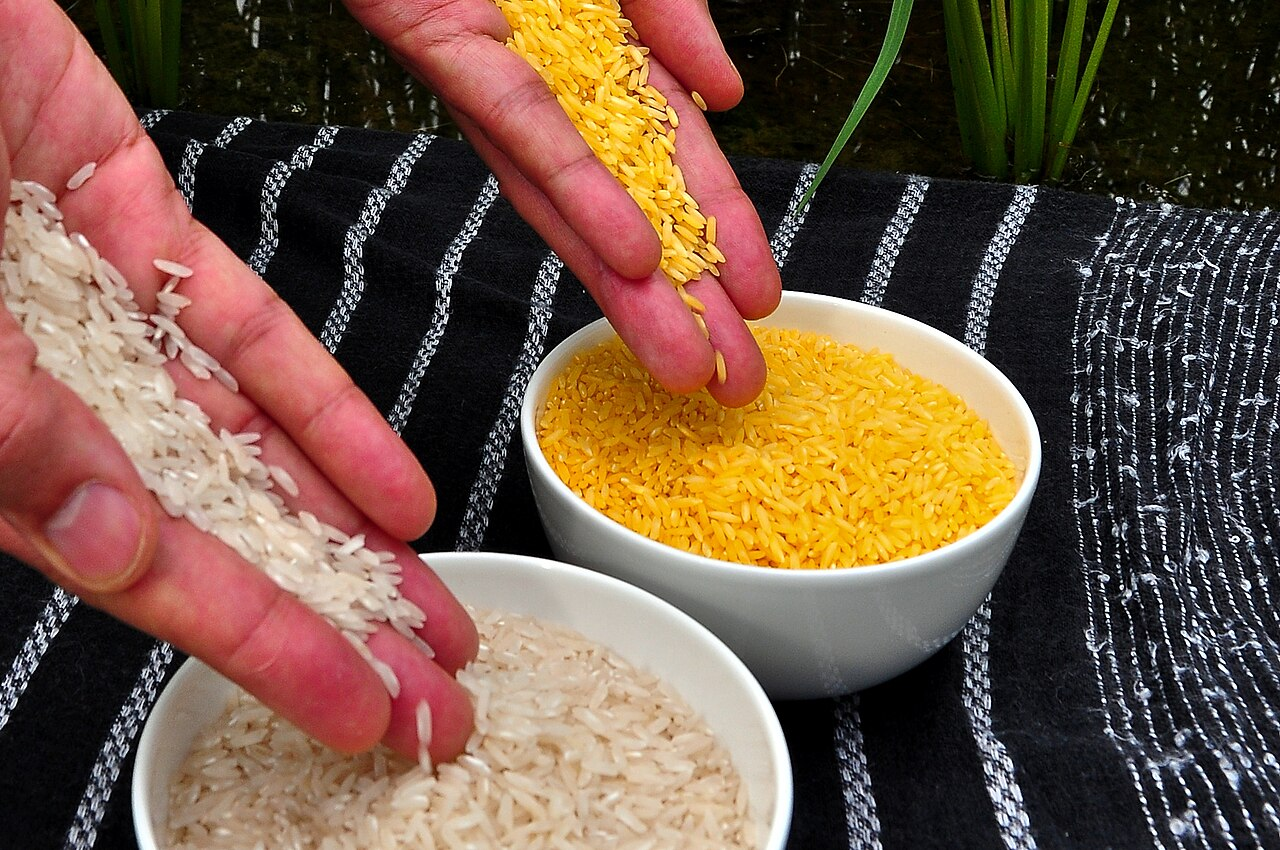
\includegraphics[width=0.46\linewidth]{images/book5/golden-rice-irri.jpg}

{\small أرز عادي وأرز ذهبي. تصنع الحبة الصفراء
$\beta$-كاروتين في سويدائها من مورّثتين مضافتين من مسلك
الكاروتينويد. يمينًا: الأرزان مقارنَين في
المعهد الدولي لبحوث الأرز (IRRI، رخصة CC~BY~2.0).}
\end{omfigure}

\begin{remark}[الجدل]\label{rem:b3:genetic-engineering:gmo}
ثلاثون سنة من الزراعة على مئات ملايين الهكتارات، وكل
مراجعة منهجية أجرتها الأكاديميات العلمية، لم تجد أي أثر
صحي للمحاصيل النقيلة المعتمدة يختلف عن
نظائرها التقليدية؛ فالمورّث \omterm{def:b3:genetic-engineering:transgenic}{النقيل} مورّثة واحدة بين أربعين
ألفًا، والبروتين الذي يصنعه يُختبر كما تُختبر أي مضافة غذائية.
أما الأسئلة الحقيقية فبيئية واقتصادية: انتشار
المقاومة في الآفات والأعشاب تحت انتقاء موحّد، وتدفق المورّثات إلى
الأقارب البرية، وتركّز سوق البذور، ومن
المستفيد. وهي الأسئلة التي تثيرها أي تقانة زراعية
قوية، وتتوقف الأجوبة على الصفة وعلى
السياق، لا على الطريقة التي نُقلت بها المورّثة.
\end{remark}

\section{تحرير الجينومات}

\begin{definition}[CRISPR--Cas9]\label{def:b3:genetic-engineering:crispr}
\index{CRISPR}\index{Cas9}\index{RNA دليل}\index{PAM}\index{تحرير الجينوم}
تخزّن البكتيريا قطعًا من جينومات العاثيات التي أصابت
أسلافها في مصفوفة من التكرارات (\emph{CRISPR})، وتستنسخها
جزيئاتِ RNA دليلة قصيرة، وتستعملها لتوجيه نوكلياز إلى قطع أي
DNA مطابق يدخل الخلية: أي منظومة مناعية تكيفية ذات
ذاكرة وراثية. وفي \emph{Streptococcus pyogenes} يكون النوكلياز
بروتينًا واحدًا هو \emph{Cas9}، يرتبط بجزيء RNA دليل وبجزيء RNA صغير
ثانٍ، ويبحث في DNA عن \emph{\omterm{def:b3:bioinformatics:motif}{نميطة} مجاورة للفاصل الأولي}
من ثلاث قواعد (PAM، أي 5$'$-NGG)، ويفك اللولب المجاور، فإذا ازدوجت
القواعد العشرون المجاورة لموقع PAM مع الدليل، قطع الطاقين على بعد ثلاث قواعد من
PAM. ولحم ينيك وشاربنتييه ودودنا وزملاؤهم (2012) جزيئي
RNA في \emph{RNA دليل واحد} وبيّنوا أن Cas9 مع دليل
بأي تسلسل مختار يقطع DNA عند ذلك التسلسل في أنبوب اختبار؛ وفي
غضون سنة تبيّن أن الزوج يعمل في خلايا الإنسان والفأر وسمك الزرد
والنبات والخميرة. و\emph{تحرير الجينوم} هو ما تفعله الخلية
بالقطع: فوصل النهايات يترك إقحامًا أو حذفًا صغيرًا
يعطّل المورّثة (أي حذف في خطوة واحدة، في أي كائن، في أسابيع)،
\omterm{def:b3:dna-repair:dsb}{وإعادة التركيب المتماثلة} مع قالب مزوَّد تكتب فيه
تسلسلًا مختارًا.
\end{definition}

\begin{omfigure}
\begin{tikzpicture}[every node/.style={font=\scriptsize}, >=stealth]
  % Cas9 outline (drawn first so labels stay on top)
  \draw[thick, omExo, fill=omExo!15] (5.9,1.1) ellipse (2.6 and 1.6);
  \node[omExo!60!black] at (7.7,2.3) {Cas9};
  % target DNA
  \draw[very thick, omDef] (0,0.3) -- (11,0.3); \draw[very thick, omDef] (0,-0.1) -- (11,-0.1);
  % PAM
  \fill[omProp!60] (7.2,-0.2) rectangle (7.9,0.4); \node[below] at (7.55,-0.25) {PAM (NGG)};
  % protospacer
  \draw[omThm, very thick] (4.2,0.5) -- (7.15,0.5); \node[above] at (5.7,0.55) {هدف من 20 قاعدة، مزدوج مع الدليل};
  % guide RNA
  \draw[very thick, omMeth!70!black] (4.2,0.3) .. controls (4.2,1.6) and (5.0,1.9) .. (5.4,1.9) -- (6.6,1.9) .. controls (7.0,1.9) and (7.2,2.5) .. (6.8,2.8) .. controls (6.3,3.1) and (5.8,2.7) .. (6.1,2.4);
  \node[left, omMeth!70!black, align=right] at (3.2,2.2) {RNA دليل واحد:\\20 قاعدة مختارة\\+ دبوس رابط للبروتين Cas9};
  % cut
  \draw[omThm, very thick, ->] (6.25,-0.7) -- (6.25,0.35); \node[omThm, below] at (6.25,-0.7) {كسر مزدوج الطاق، على بعد 3 قواعد من PAM};
  % outcomes
  \draw[->, thick] (2.0,-1.3) -- (2.0,-1.9); \node[below, align=center] at (2.0,-1.9) {وصل النهايات:\\إقحام أو حذف صغير\\$\Rightarrow$ إزاحة إطار، وحذف};
  \draw[->, thick] (10.0,-1.3) -- (10.0,-1.9); \node[below, align=center] at (10.0,-1.9) {إعادة تركيب مع\\قالب مزوَّد\\$\Rightarrow$ تغير دقيق};
\end{tikzpicture}

{\small \omterm{def:b3:genetic-engineering:crispr}{Cas9} ودليله. يرتبط البروتين بموقع \omterm{def:b3:genetic-engineering:crispr}{PAM}، ويفك DNA
المجاور لها، ويقطع إذا ازدوجت القواعد العشرون مع \omterm{def:b3:genetic-engineering:crispr}{RNA الدليل}.
ويُصلَح الكسر إما بوصل النهايات، فيعطّل المورّثة، وإما
بإعادة تركيب مع قالب، فيعيد كتابتها.}
\end{omfigure}

\begin{proposition}[التحرير بلا كسر]\label{prop:b3:genetic-engineering:editors}
\index{محرّر قواعد}\index{محرّر أوّلي}\index{خارج الهدف}
قطع الطاقين أخشن ضروب التحرير: فنتيجة وصل النهايات
عشوائية، والكسر في موضع آخر --- أي موقع \emph{\omterm{prop:b3:genetic-engineering:editors}{خارج الهدف}} يختلف
عن الدليل في مواضع قليلة يتسامح معها \omterm{def:b3:genetic-engineering:crispr}{Cas9} --- طفرة
لم يطلبها أحد. \omterm{def:b3:genetic-engineering:crispr}{وCas9} المعطَّل أحد نطاقي النوكلياز فيه
يثلم طاقًا واحدًا؛ والمعطَّل كلاهما يرتبط فحسب، ويستطيع أن
يحمل إنزيمات أخرى إلى متتالية. و\emph{محرّرات القواعد} تلحم
\omterm{def:b3:genetic-engineering:crispr}{Cas9} الثالم بنازع أمين يحوّل C إلى U (تُقرأ T) أو A إلى I
(تُقرأ G) في الطاق المفكوك، فتغيّر قاعدة واحدة بلا كسر
وبلا قالب؛ و\emph{المحرّرات الأولية} تحمل ناسخًا
عكسيًا ودليلًا مطوَّلًا بالتسلسل المرغوب، فتنسخ
ذلك التسلسل في الطاق المثلوم، فتتيح أي استبدال
وإقحامات أو حذوف صغيرة. ويُخفَّض النشاط \omterm{prop:b3:genetic-engineering:editors}{خارج الهدف}
بصور \omterm{def:b3:genetic-engineering:crispr}{Cas9} المهندسة عالية الأمانة، وبإيصال الإنزيم
عابرًا بروتينًا لا مورّثةً، وباختيار أدلة يختلف
أقرب أقاربها الجينوميين عنها في عدة مواضع؛ ويُقاس
بتسلسل المواقع المتوقعة، وبطرائق غير منحازة تلتقط
كل كسر في الجينوم.
\end{proposition}

\begin{example}[شفاء]\label{ex:b3:genetic-engineering:sickle}
فقر الدم المنجلي تغيرُ قاعدة واحدة في الغلوبين $\beta$. والهيموغلوبين
الجنيني، المصنوع من الغلوبين $\gamma$، كان ليحل محله، لكن
مورّثات $\gamma$ تُطفأ بعد الولادة بالكابح BCL11A.
وأول علاج معتمد بمنظومة \omterm{def:b3:genetic-engineering:crispr}{CRISPR} (2023) يأخذ خلايا الدم الجذعية
من المريض نفسه، ويقطع المعزِّز الحمراوي في \emph{BCL11A} بالبروتين \omterm{def:b3:genetic-engineering:crispr}{Cas9} حتى
يعطّله وصل النهايات في معظم الخلايا، ويعيد الخلايا بعد
تفريغ نقي المريض: فتكون الكريات الحمر التي تصنعها غنية
بالهيموغلوبين الجنيني، ولا تتمنجل، وتتوقف النوب. والتحرير
جسدي --- فالسلالة الجنسية لم تُمسّ والتغير لا يُورَّث
--- وهو يستعمل النتيجة ``الخشنة''، أي التعطيل، حيث يكون التعطيل
هو المطلوب.
\end{example}

\begin{theorem}[الانتشار فوق المندلي لدافع مورّثي]\label{thm:b3:genetic-engineering:drive}
\index{دافع مورّثي}
\emph{\omterm{thm:b3:genetic-engineering:drive}{الدافع المورّثي}} بنية تشفّر \omterm{def:b3:genetic-engineering:crispr}{Cas9} ودليلًا يقطع
الأليل البري عند موضعه هو في متغاير اللواقح؛ فيعيد الإصلاح
بإعادة التركيب نسخ الدافع في الصبغي المقطوع، فتحمل
نسبة $c$ من أعراس متغاير اللواقح الدافعَ بدل
النصف المندلي. فإذا كان تواتر الدافع $p$ في جمهرة كبيرة
تتزاوج عشوائيًا بلا كلفة لياقة، كان تواتره في
الجيل التالي
\[
p' = p + c\,p\,(1 - p),
\]
فينتشر من الندرة بمعدل يتناسب مع $c$، ويبلغ
نصف الجمهرة في نحو $\ln(1/p_{0})/\ln(1 + c)$
جيلًا انطلاقًا من تواتر ابتدائي $p_{0}$.
\end{theorem}
\begin{proof}
يعطي التزاوج العشوائي متماثلات اللواقح للدافع بتواتر $p^{2}$،
ومتغايرات اللواقح بتواتر $2p(1-p)$، ومتماثلات اللواقح البرية بتواتر $(1-p)^{2}$. و
متماثلات اللواقح تنقل الدافع إلى كل أعراسها، ومتغايرات اللواقح
إلى نسبة $(1 + c)/2$ (نصف بمندل، زائدًا $c$ مضروبًا في النصف
البري المحوَّل)، والبرية إلى لا شيء. ومنه $p' = p^{2} + 2p(1-p)(1+c)/2
= p^{2} + p(1-p) + c\,p(1-p) = p + c\,p(1-p)$. ومن أجل $p$ صغيرة يكون هذا
$p' \approx (1+c)p$، أي نموًا هندسيًا بنسبة $1 + c$، يبلغ
$1/2$ من $p_{0}$ بعد نحو $\ln(1/2p_{0})/\ln(1+c)$ جيلًا؛ أما
الحد اللوجستي فلا يبطئه إلا قرب النهاية.
\end{proof}

\begin{omfigure}
\begin{tikzpicture}
\begin{axis}[
  width=0.7\linewidth, height=5.6cm,
  axis x line=bottom, axis y line=left,
  xmin=0, xmax=20, ymin=0, ymax=1.05,
  xlabel={الجيل}, ylabel={تواتر الدافع $p$},
  xlabel style={font=\small, at={(axis description cs:0.5,-0.12)}, anchor=north},
  ylabel style={font=\small},
  tick label style={font=\small}, xtick={0,5,10,15,20}, ytick={0,0.5,1},
  clip=false,
]
\addplot[very thick, omThm, mark=*, mark size=1.2pt] coordinates {(0,0.01) (1,0.0189) (2,0.0356) (3,0.0665) (4,0.1224) (5,0.2191) (6,0.3731) (7,0.5836) (8,0.8023) (9,0.9451) (10,0.9918) (11,0.9991) (12,1.0) (13,1.0) (14,1.0) (15,1.0) (16,1.0) (17,1.0) (18,1.0) (19,1.0) (20,1.0)};
\addplot[very thick, omDef, mark=*, mark size=1.2pt] coordinates {(0,0.01) (1,0.015) (2,0.0223) (3,0.0332) (4,0.0493) (5,0.0727) (6,0.1064) (7,0.154) (8,0.2191) (9,0.3047) (10,0.4106) (11,0.5316) (12,0.6561) (13,0.769) (14,0.8578) (15,0.9188) (16,0.9561) (17,0.9771) (18,0.9883) (19,0.9941) (20,0.997)};
\addplot[very thick, gray, dashed, domain=0:20, samples=2] {0.01};
\node[font=\scriptsize, omThm, anchor=south east] at (axis cs:6.5,0.62) {$c = 0.9$};
\node[font=\scriptsize, omDef, anchor=north west] at (axis cs:12.5,0.62) {$c = 0.5$};
\node[font=\scriptsize, gray, anchor=south west] at (axis cs:12,0.02) {مندلي، $c = 0$: يبقى عند $p_{0}$};
\end{axis}
\end{tikzpicture}

{\small \omterm{thm:b3:genetic-engineering:drive}{دافع مورّثي} أُطلق عند واحد في المئة، بكفاءة تحويل
$0.9$ أو $0.5$ وبلا كلفة لياقة. والأليل المندلي بلا
أفضلية كان ليبقى عند واحد في المئة؛ أما الدافع فيستولي في عشرة
أجيال أو عشرين.}
\end{omfigure}

\begin{remark}[ما الذي يجوز تحريره]\label{rem:b3:genetic-engineering:ethics}
تحرير الخلايا الجسدية لمريض موافق طبٌّ، يُحكم
عليه كأي علاج بمخاطره ومنافعه. أما تحرير السلالة الجنسية ---
أي جنين يحمل كل خلف له التغيرَ --- فمختلف
في النوع: فالشخص المتأثر لا يستطيع أن يوافق، والتغير
يُورَّث، ونتائج التقنية \omterm{prop:b3:genetic-engineering:editors}{خارج الهدف} والفسيفسائية لم تُضبط
بعد؛ وبعد أن أعلن عالم صيني عام 2018 أنه
فعل ذلك في توأمين، دعت الأكاديميات العلمية في معظم البلدان
إلى وقف مؤقت وجرّمته عدة دول. \omterm{thm:b3:genetic-engineering:drive}{والدافع المورّثي}
المطلق في جمهرة برية قرار يُتخذ عن كل من
يأتي بعد، ولهذا تقرن مقترحات هذا الحقل نفسه للقضاء على
بعوض الملاريا الدوافعَ بصمامات أمان --- دوافع عكسية،
وتصاميم ذاتية التحديد --- وبموافقة عامة في البلدان
المعنية.
\end{remark}

\section{تمارين}

\begin{exercise}[$\star$]\label{exo:b3:genetic-engineering:1}
اذكر المكونات الثلاثة التي يجب أن تكون في \omterm{def:b3:genetic-engineering:tools}{بلازميد} استنساخ وفسّر
غرض كل منها.
\end{exercise}

\begin{exercise}[$\star$]\label{exo:b3:genetic-engineering:2}
يتعرف EcoRI المتتالية GAATTC. فكم مرة يرد الموقع وسطيًا في
DNA عشوائي، وكم قطعة يصنع من جينوم \emph{E.~coli} البالغ
\qty{4.6}{Mb}؟ ولماذا يختلف العدد الحقيقي بعض الشيء؟
\end{exercise}

\begin{exercise}[$\star$]\label{exo:b3:genetic-engineering:3}
اذكر خطوات الحرارة الثلاث في دورة PCR وما يحدث عند
كل منها. ولماذا يجب أن يكون البوليميراز ثابتًا حراريًا؟
\end{exercise}

\begin{exercise}[$\star$]\label{exo:b3:genetic-engineering:4}
ما الذي يحتاجه \omterm{def:b3:genetic-engineering:crispr}{Cas9} ليقطع متتالية معينة، وما النتيجتان
اللتان يمكن أن تتبعا القطع؟
\end{exercise}

\begin{exercise}[$\star\star$]\label{exo:b3:genetic-engineering:5}
يعمل تفاعل PCR $35$ دورة بكفاءة $E = 0.9$ من $50$ نسخة. فكم
نسخة تنتج؟ ويعطي تفاعل qPCR لعينتين $C_{T} = 18.2$ و$25.5$؛
فما نسبة كميتيهما الابتدائيتين عند $E = 0.95$؟
\end{exercise}

\begin{exercise}[$\star\star$]\label{exo:b3:genetic-engineering:6}
لماذا تُستعمل مكتبة cDNA لا مكتبة جينومية للتعبير عن
بروتين بشري في البكتيريا؟ سمِّ عقبتين أخريين أمام صنع بروتين
بشري في \emph{E.~coli} وقل كيف تُتجاوز كل منهما.
\end{exercise}

\begin{exercise}[$\star\star$]\label{exo:b3:genetic-engineering:7}
يُصنع فأر محذوف المورّثة \omterm{def:b3:genetic-engineering:transgenic}{باستهداف مورّثي} في خلايا جذعية جنينية.
فسّر لماذا يكون أول فأر يولد خيمريًا، ولماذا يجب تزويجه،
وما نسبة أحفاد الخيمري الذي نصف سلالته الجنسية مستهدَفة
الذين يكونون متماثلي اللواقح للحذف إذا زُوّج الأجداد متغايرو
اللواقح فيما بينهم.
\end{exercise}

\begin{exercise}[$\star\star$]\label{exo:b3:genetic-engineering:8}
يُختار \omterm{def:b3:genetic-engineering:crispr}{RNA دليل} من 20 قاعدة مع \omterm{def:b3:genetic-engineering:crispr}{PAM} من نمط NGG. فكم موقعًا في
جينوم قدره $3.2\times 10^{9}$ زوج قواعد (على الطاقين) يطابق الدليل تمامًا
مصادفةً؟ وكم موقعًا يطابقه بعدم توافق في موضعين على الأكثر، إذا تسامح \omterm{def:b3:genetic-engineering:crispr}{Cas9}
معهما؟ (عُدّ المتتاليات ضمن عدم توافق في موضعين بأنها $1 + 3\binom{20}{1} +
9\binom{20}{2}$.)
\end{exercise}

\begin{exercise}[$\star\star$]\label{exo:b3:genetic-engineering:9}
باستعمال \cref{thm:b3:genetic-engineering:drive}، احسب تواتر
دافع عند $c = 0.8$ بعد ثلاثة أجيال من $p_{0} = 0.05$، و
قدّر عدد الأجيال لبلوغ $0.5$.
\end{exercise}

\begin{exercise}[$\star\star\star$]\label{exo:b3:genetic-engineering:10}
علاج فقر الدم المنجلي يعطّل معزِّزًا بدل أن يصحح طفرة
الغلوبين $\beta$. أعطِ سببين لاختيار التعطيل بوصل النهايات
على التصحيح \omterm{def:b3:dna-repair:dsb}{بإعادة التركيب المتماثلة} في خلايا الدم الجذعية،
وعيبًا واحدًا.
\end{exercise}

\begin{exercise}[$\star\star\star$]\label{exo:b3:genetic-engineering:11}
\omterm{thm:b3:genetic-engineering:drive}{دافع مورّثي} ضد بعوضة يحمل كلفة لياقة $s$ في
متماثلات اللواقح. عدّل علاقة التكرار لتشمل الانتقاء ضد متماثلات
اللواقح للدافع وأوجد الشرط على $c$ وَ$s$ لينتشر الدافع
من الندرة. ثم فسّر لماذا تكون أليلات المقاومة --- أي نواتج وصل
النهايات عند الهدف التي لم يعد الدليل يتعرفها --- هي
العقبة الرئيسة عمليًا.
\end{exercise}

\begin{exercise}[$\star\star\star$]\label{exo:b3:genetic-engineering:12}
احتجّ، بآليات هذا الفصل وآليات
\cref{ch:b3:dna-repair}، على أن تحرير السلالة الجنسية لجنين بشري لا
يستطيع في الوقت الحاضر أن يضمن النتيجة المقصودة في كل خلية، وأي
دليل يلزم قبل أن يستطيع عاقل أن يعدّه
آمنًا.
\end{exercise}

\section{مسألة: من مورّثة إلى دواء ومحصول}

\begin{problem}[{مسألة نهاية الأسبوع --- مورّثة مستنسخة بحساب
مواقع القطع والتحول، وفيروس معدود بتفاعل qPCR، و
هرمون يُنتج بالأطنان في مخمّرة، وجينوم محرَّر مع عدّ
مواقعه خارج الهدف، ودافع مورّثي موقوت، وتنتهي إلى نسخ
فيروس في عينة، وحجم المخمّرة السنوي لأنسولين العالم
وعدد الأجيال التي يحتاجها دافع}]
\label{pb:b3:genetic-engineering:1}
معطيات: مورّثة بطول \qty{1.5}{kb}؛ وموقع قطع من ست قواعد؛ \omterm{def:b3:genetic-engineering:tools}{وبلازميد}
بطول \qty{4}{kb}؛ وكفاءة تحول $2\times 10^{7}$ مستعمرة لكل
ميكروغرام من \omterm{def:b3:genetic-engineering:tools}{البلازميد}؛ والوصل يعطي \qty{10}{\%} من البلازميدات
مقحَمة. وكفاءة qPCR هي $E = 1$، والعتبة $N_{T} = 10^{12}$. والأنسولين:
\qty{5.8}{kDa}، ويستعمل المريض $40$ وحدة في اليوم، والوحدة
\qty{35}{\micro g}؛ و$10^{7}$ مريض؛ وتعطي المخمّرة
\qty{2}{g/L} من الناتج في الدفعة، وعشر دفعات في السنة. والجينوم $3.2\times
10^{9}$ زوج قواعد. وتحويل الدافع $c = 0.9$، مطلَقًا عند $p_{0} = 0.001$.

\medskip
\noindent\textbf{الجزء الأول --- الاستنساخ.}
\begin{enumerate}
  \item كم مرة يرد موقع معين من ست قواعد في DNA عشوائي؟ وما
        احتمال ألا تحوي المورّثة البالغة \qty{1.5}{kb} أي موقع
        كهذا، فيمكن استعمال الإنزيم لاستنساخها كاملةً؟
  \item وإذا حوت موقعًا، فكيف تستنسخها مع ذلك؟
        (طريقتان.)
  \item يُحوَّل \qty{100}{ng} من \omterm{def:b3:genetic-engineering:tools}{البلازميد} الموصول. فكم
        مستعمرة، وكم منها يحمل المقحَمة؟
  \item يُستعمل الفرز الأزرق والأبيض. فما نسبة المستعمرات
        البيضاء، وكم مستعمرة بيضاء يجب التقاطها ليكون احتمال أن
        تحمل واحدة منها على الأقل المورّثة بالاتجاه
        الصحيح \qty{99}{\%} (ونصف المقحمات بالاتجاه الصحيح)؟
  \item \omterm{def:b3:genetic-engineering:tools}{البلازميد} المؤتلف \qty{5.5}{kb}. وتحوي الخلية $50$
        نسخة وتنقسم كل \qty{30}{min}. فبعد نمو ليلة
        (\qty{16}{h}) من خلية واحدة، كم جزيء \omterm{def:b3:genetic-engineering:tools}{بلازميد}، و
        ما كتلة DNA البلازميدي (\qty{650}{Da} لكل زوج قواعد)؟
  \item لماذا يحتاج \omterm{def:b3:genetic-engineering:tools}{البلازميد} إلى منشأ بكتيري بينما لا تحتاج
        المورّثة البشرية المقحَمة إلى مروّج بكتيري للاستنساخ،
        وتحتاج إليه للتعبير؟
\end{enumerate}

\medskip
\noindent\textbf{الجزء الثاني --- عدّ فيروس.}
\begin{enumerate}[resume]
  \item تعبر عينة مريض العتبة عند $C_{T} = 28$. فكم
        نسخة كانت في التفاعل؟ وأخرى عند $C_{T} = 35$؟
  \item الحساسية: كم دورة تلزم لإيصال نسخة واحدة
        إلى العتبة؟
  \item تُضبط عتبة قطع الاختبار عند $C_{T} = 38$. فأي عدد من
        النسخ يوافق ذلك، ولماذا لا تُستعمل $45$ دورة؟
  \item يدخل جزيء ملوث من ناتج شوط سابق عينةً
        سلبية. فعند أي دورة يعبر العتبة؟
        وأي ممارسة مخبرية تمنع ذلك؟
  \item يحوّل النسخ العكسي \qty{40}{\%} من RNA الفيروسي إلى
        DNA. صحّح عدّ السؤال 7 للعينة الأولى.
  \item تختلف عينتان بمقدار $\Delta C_{T} = 3.3$ عند $E = 1$، لكن
        الكفاءة في الواقع $0.9$. فما الفرق الذي يبلّغ عنه
        المحلل، وما الفرق الحقيقي؟
\end{enumerate}

\medskip
\noindent\textbf{الجزء الثالث --- الأنسولين بالأطنان.}
\begin{enumerate}[resume]
  \item احسب كتلة الأنسولين اليومية لكل مريض والحاجة
        العالمية السنوية لعدد $10^{7}$ مريض، بالكيلوغرامات.
  \item كم مولًا من الأنسولين ذلك، وكم جزيئًا؟
  \item أي حجم مخمّرة، بعشر دفعات في السنة، ينتجه؟
        قارنه بمسبح حجمه \qty{2500}{m^3}.
  \item أعطى الاستخلاص من الغدد \qty{1}{kg} من الأنسولين لكل
        \qty{8000}{kg} من البنكرياس؛ وبنكرياس الخنزير يزن
        \qty{100}{g}. فكم خنزيرًا يحتاج العالم في السنة؟
  \item لماذا يُفضَّل الهرمون المؤتلف حتى حيث يكون الأنسولين
        الحيواني رخيصًا؟ أعطِ سببين.
  \item تختلف نظائر الأنسولين عن التسلسل البشري ببقية أو
        اثنتين. فسّر لماذا يبقى النظير دواءً يعمل على
        المستقبل البشري، ولماذا يغيّر تبديل بقية واحدة
        زمن تفككه.
\end{enumerate}

\medskip
\noindent\textbf{الجزء الرابع --- التحرير والدفع.}
\begin{enumerate}[resume]
  \item كم مطابقة تامة لدليل من 20 قاعدة مع \omterm{def:b3:genetic-engineering:crispr}{PAM} من نمط NGG يحوي
        الجينوم مصادفةً (على الطاقين: $6.4\times 10^{9}$
        موضع)؟
  \item إذا تسامح \omterm{def:b3:genetic-engineering:crispr}{Cas9} مع عدم توافق في ثلاثة مواضع على الأكثر، فكم متتالية
        تقع ضمن ثلاثة مواضع من الدليل، وكم موقعًا مصادفًا \omterm{prop:b3:genetic-engineering:editors}{خارج الهدف} ينتج؟
  \item الخلايا الدموية الجذعية المحرَّرة $10^{7}$؛ و\qty{80}{\%} منها تحمل
        التعطيل المقصود. فكم خلية تحمل كسرًا \omterm{prop:b3:genetic-engineering:editors}{خارج الهدف}
        عند موقع معين إذا قُطع في خلية واحدة من $10^{4}$،
        ولماذا يقلق كسرٌ في مورّثة كابحة للورم في خلية جذعية
        واحدة؟
  \item احسب تواتر الدافع بعد $1, 2, 3$ أجيال من
        $p_{0} = 0.001$، وقدّر الأجيال حتى $0.5$.
  \item للبعوضة عشرة أجيال في السنة. فكم سنة يحتاج ليستولي؟
        وكيف تغيّر كلفةُ لياقة قدرها \qty{20}{\%} في متماثلات اللواقح
        الصورةَ نوعيًا؟
  \item ينشأ أليل مقاومة حين يصلح الكسرَ وصلُ النهايات لا إعادة التركيب،
        باحتمال $1 - c = 0.1$ لكل محاولة تحويل. قدّر عدد
        أليلات المقاومة المتولدة في جمهرة من $10^{6}$ متغاير لواقح في جيل واحد،
        وفسّر ما الذي يحدث للدافع إذا كانت لائقة.
  \item لخّص: النسخ في العينة الأولى (السؤال~7)، وحجم
        مخمّرة الأنسولين العالمي السنوي (السؤال~15)، و
        الأجيال التي يبلغ فيها الدافع نصف الجمهرة
        (السؤال~22).
\end{enumerate}
\end{problem}
